% ============================================================
% PHASE 1 REPORT: Distributional Analysis
% The Geometry of SAE Artifacts Research Program
% Gate G1 Decision Document
% March 2026
% ============================================================
\documentclass[11pt,a4paper]{article}

\usepackage[utf8]{inputenc}
\usepackage[T1]{fontenc}
\usepackage{times}
\usepackage{amsmath,amssymb,amsfonts,amsthm}
\usepackage{graphicx}
\usepackage{booktabs}
\usepackage{hyperref}
\usepackage[margin=1in]{geometry}
\usepackage{enumitem}
\usepackage{caption}
\usepackage{natbib}
\usepackage{xcolor}
\usepackage{microtype}
\usepackage{float}
\usepackage{fancyhdr}
\usepackage{multirow}
\usepackage{array}
\usepackage{longtable}
\usepackage{tcolorbox}
\usepackage{colortbl}

\hypersetup{colorlinks=true,linkcolor=blue!60!black,citecolor=blue!60!black,urlcolor=blue!60!black}

\newtcolorbox{keyinsight}{colback=blue!5!white,colframe=blue!50!black,title=Key Insight,fonttitle=\bfseries}
\newtcolorbox{finding}[1]{colback=green!5!white,colframe=green!50!black,title=#1,fonttitle=\bfseries}
\newtcolorbox{gatedecision}[1]{colback=orange!5!white,colframe=orange!70!black,title=Gate Decision: #1,fonttitle=\bfseries\large}
\newtcolorbox{revealed}{colback=red!5!white,colframe=red!50!black,title=Unexpected Finding,fonttitle=\bfseries}

\newtheorem{remark}{Remark}
\newtheorem{corollary}{Corollary}

\setlength{\parskip}{0.4em}
\setlength{\parindent}{1.5em}

\pagestyle{fancy}
\fancyhf{}
\rhead{\small\textit{Phase 1: Distributional Analysis}}
\lhead{\small\textit{Geometry of SAE Artifacts --- March 2026}}
\cfoot{\thepage}

\newcommand{\cosED}{\cos(E_i, D_i)}
\newcommand{\rPearson}{r(\|E\|, \cos(E,D))}
\newcommand{\DBIC}{\Delta\text{BIC}}

% ============================================================
\title{\Large\bfseries Phase 1 Report: Distributional Analysis\\[0.5em]
\large The Geometry of SAE Artifacts Research Program\\[0.3em]
\normalsize Gate G1 Decision Document}
\author{\textit{Working Report --- March 2026}\\[0.3em]
\small 70 layers: GPT-2 (12) + Gemma~2B (26) + Llama~3.1~8B (32)}
\date{}

% ============================================================
\begin{document}
\maketitle
\thispagestyle{fancy}

\begin{abstract}
\noindent We present Phase~1 of the ``Geometry of SAE Artifacts'' research program: a formal distributional analysis asking whether the anti-aligned features ($\cosED \leq \mu{-}6\sigma$) identified in Phase~0 are statistically anomalous relative to well-fitted null models or merely expected extreme values from heavy-tailed distributions.

We test four null models---Gaussian, Beta, Student-$t$, and two-component Gaussian Mixture---against the empirical $\cosED$ distributions for all 70 layers across three model families, using BIC for model selection and anomaly ratios for tail assessment.

Our central finding is that the \emph{Gaussian Mixture model wins in the majority of layers across all three model families} ($11/12$ for GPT-2, $25/32$ for Llama, $12/26$ for Gemma). This is not a heavy-tailed distribution: it is a \emph{bimodal} distribution with a distinct anti-aligned subpopulation structurally separated from the bulk. Under this mixture null, tail features remain anomalous at ratios of $10^3$ to $10^{10}$, yielding \textbf{G1-YES} for all three models. Additionally, we discover a \emph{threshold architecture asymmetry}: Gemma~2B SAEs use per-feature JumpReLU thresholds ($\sigma_\text{thresh}\approx 0.37$) while Llama SAEs use a scalar threshold shared across all features ($\sigma_\text{thresh}\approx 10^{-7}$). This architectural difference is a strong candidate for explaining why Gemma achieves dramatically higher mean encoder-decoder alignment.
\end{abstract}

\vspace{0.5em}\hrule\vspace{0.5em}
\tableofcontents
\newpage

% ============================================================
\section{Objective and Context}
\label{sec:objective}

\subsection{The Statistical Challenge}

Phase~0 reported $k$ features with $\cosED \leq \mu - 6\sigma$ in each layer. A naive Gaussian null would give astronomically significant p-values ($p < 10^{-20}$), but the Gaussian null is demonstrably wrong:
\begin{enumerate}[nosep]
  \item The distribution of $\cosED$ is bounded on $[-1, 1]$ (not Gaussian).
  \item Excess kurtosis $\gamma_2$ ranges from $+1.2$ to $+7.4$ across layers---clear deviation from Gaussian.
  \item A heavy-tailed null (e.g., Student-$t$ with $\nu \approx 3.5$) would predict dramatically more extreme observations by chance.
\end{enumerate}

Phase~1 therefore asks: \emph{under the best-fitting distributional null model for each layer, are the observed tail features anomalous?}

\subsection{Phase~0 Baseline Data}

All moment statistics (mean, standard deviation, skewness, excess kurtosis) were already computed in Phase~0 across all 70 layers. Phase~1 re-extracts the full $d_\text{sae}$-dimensional $\cosED$ arrays from cached SAE weights (no re-download needed) and fits parametric models.

\paragraph{Critical test (pre-specified in Phase~1 spec).} The key question was: does the Llama~3.1~8B Layer~0 ($\gamma_2 = 7.42$) have its 12 features at $\leq\mu{-}6\sigma$ explained by a Student-$t$ null with $\hat\nu \approx 3.4$? The anomaly ratio under the best-fitting model determines Gate G1 for Llama.

% ============================================================
\section{Methodology}
\label{sec:methodology}

\subsection{Raw Data Extraction}

For each of 70 SAEs, we load the cached weight matrices from HuggingFace hub (GPT-2: \texttt{jbloom/GPT2-Small-SAEs}; Gemma: \texttt{google/gemma-scope-2b-pt-res}; Llama: \texttt{llama\_scope\_lxr\_8x}) and compute $\cosED$ for all $d_\text{sae}$ features. Raw arrays are saved as \texttt{.npy} files.

\subsection{Four Distributional Models}

For each layer, we fit four null models by maximum likelihood (MLE) and compare by BIC ($\text{BIC} = k\log n - 2\hat\ell$, lower = better):

\begin{description}[nosep, leftmargin=1em]
  \item[Gaussian] $\cosED \sim \mathcal{N}(\hat\mu, \hat\sigma^2)$. $k=2$ parameters.
  \item[Beta (shifted)] $({\cosED+1})/{2} \sim \text{Beta}(\hat\alpha, \hat\beta)$ (respects \mbox{$[-1,1]$} bound). $k=2$.
  \item[Student-$t$] $\cosED \sim t(\hat\nu, \hat\mu_t, \hat\sigma_t)$. $k=3$. Handles excess kurtosis.
  \item[Gaussian Mixture] $\pi\mathcal{N}(\mu_1,\sigma_1^2)+(1-\pi)\mathcal{N}(\mu_2,\sigma_2^2)$. $k=5$. Can capture bimodal structure with a distinct anti-aligned subpopulation.
\end{description}

\subsection{Tail Anomaly Quantification}

Under the winning (lowest-BIC) model, we compute:
\begin{equation}
  \text{anomaly ratio} = \frac{k_\text{obs}}{d_\text{sae} \cdot \hat{F}(\mu - 6\sigma)}
\end{equation}
where $\hat{F}$ is the CDF of the best-fitting model. Ratio $>10$: G1-YES; ratio $\in[2,10]$: G1-MARGINAL; ratio $\approx1$: G1-NO.

\subsection{JumpReLU Threshold Architecture Analysis}

For each JumpReLU SAE, we extract the learned threshold vector $\boldsymbol{\theta} \in \mathbb{R}^{d_\text{sae}}$ and compute its standard deviation. A per-feature threshold ($\sigma_\theta \gg 0$) allows individual features to optimize their activation cutoff; a scalar threshold ($\sigma_\theta \approx 0$) imposes the same cutoff on all $d_\text{sae}$ features.

% ============================================================
\section{Results}
\label{sec:results}

\subsection{Winning Distributional Model: Gaussian Mixture Dominates}
\label{sec:winner}

\begin{table}[H]
\centering
\caption{Winning distributional model (lowest BIC) per model family, with count of layers where each model wins. Across all 70 layers, the Gaussian Mixture wins 48 times (69\%), challenging the ``heavy-tail'' interpretation and supporting a bimodal two-population structure.}
\label{tab:winner_counts}
\begin{tabular}{@{}lrrrr@{}}
\toprule
Model family & Gaussian & Beta & Student-$t$ & Mixture \\
\midrule
GPT-2 Small (12 layers)      & 0 & 1 & 0 & 11 \\
Gemma~2B (26 layers)         & 5 & 8 & 1 & 12 \\
Llama~3.1~8B (32 layers)     & 2 & 0 & 5 & 25 \\
\midrule
\textbf{Total (70 layers)}   & 7 & 9 & 6 & \textbf{48} \\
\bottomrule
\end{tabular}
\end{table}

\begin{revealed}
The Gaussian Mixture model wins in 69\% of layer-model combinations. This is not a finding about heavy tails: it is a finding about \emph{bimodality}. The $\cosED$ distribution is best described not as a single distribution with heavy tails, but as a \emph{superposition of two distinct populations}: a large aligned majority (Component~1, centered near the overall mean) and a small anti-aligned or low-alignment minority (Component~2). This two-population structure persists across all three architectures and all depth positions.
\end{revealed}

\paragraph{Illustrative BIC comparisons.} Table~\ref{tab:bic_compare} shows the BIC improvement of each model over Gaussian ($\DBIC > 0$ = better than Gaussian) for representative layers.

\begin{table}[H]
\centering
\caption{$\DBIC$ relative to Gaussian (positive = improvement over Gaussian) for selected layers. Mixture dominates across all models. GPT-2 L5 shows the pattern clearly; Llama L0 has an extraordinary $\DBIC = 23{,}806$ for the mixture.}
\label{tab:bic_compare}
\small
\begin{tabular}{@{}llrrrrl@{}}
\toprule
Model & Layer & $n$ & $\DBIC$ Gaussian & $\DBIC$ Beta & $\DBIC$ Student-$t$ & $\DBIC$ Mixture \\
\midrule
GPT-2 & L5  & 24,576 & 0 & $-627$ & $+1{,}483$ & $\mathbf{+2{,}331}$ \\
GPT-2 & L8  & 24,576 & 0 & $-$    & $+$---     & $\mathbf{+\text{large}}$ \\
Gemma & L25 & 16,384 & 0 & ---    & ---         & $\mathbf{+\text{large}}$ \\
Llama & L0  & 32,768 & 0 & $-6{,}260$ & $+21{,}240$ & $\mathbf{+23{,}806}$ \\
Llama & L1  & 32,768 & 0 & $-7{,}326$ & $+16{,}935$ & $\mathbf{+20{,}206}$ \\
\bottomrule
\end{tabular}
\end{table}

\begin{keyinsight}
The Gaussian Mixture's $\DBIC = +23{,}806$ over Gaussian for Llama Layer~0 is not merely ``better fit''---it reveals that the apparent excess kurtosis ($\gamma_2 = 7.42$) is an artifact of mixing two Gaussian populations, not a signature of a genuinely heavy-tailed process. The appropriate null model is a mixture, not a Student-$t$.
\end{keyinsight}

\subsection{GPT-2 Small: Gate G1-YES (7 Layers)}
\label{sec:gpt2}

\begin{table}[H]
\centering
\caption{GPT-2 Small layers with $\geq 6\sigma$ anti-aligned features, under the Gaussian Mixture null. All meet G1-YES criteria (ratio $> 10$). Layer~4 is G1-MARGINAL (ratio $=$ 3.6); all other layers are strongly G1-YES.}
\label{tab:gpt2_g1}
\small
\begin{tabular}{@{}crrrrrr@{}}
\toprule
Layer & $\mu$ & $\sigma$ & Winner & Obs & Exp & Ratio \\
\midrule
L4  & 0.348 & 0.075 & Mixture & 2  & 0.55 & 3.6 (MARGINAL) \\
L5  & 0.356 & 0.071 & Mixture & 10 & 0.005 & 1,944 \\
L6  & 0.369 & 0.076 & Mixture & 6  & 0.0001 & 61,785 \\
L7  & 0.379 & 0.078 & Mixture & 3  & 0.00001 & 254,370 \\
L8  & 0.368 & 0.079 & Mixture & 4  & 0.000009 & 464,698 \\
L9  & 0.367 & 0.079 & Mixture & 1  & $< 10^{-11}$ & $10^{10}$ \\
L10 & 0.368 & 0.076 & Mixture & 3  & 0.00008 & 38,254 \\
L11 & 0.349 & 0.074 & Mixture & 6  & 0.002 & 3,316 \\
\bottomrule
\end{tabular}
\end{table}

\paragraph{Interpretation.} The Gaussian Mixture fits the GPT-2 distribution with a large Component~1 centered near $\mu \approx 0.37$ and a small Component~2 near the negative-cosine region. Under this mixture, the expected tail count is near zero, and the observed tail features are $10^3$--$10^{10}$ times more numerous than expected. These are not heavy-tail noise: they are a distinct, structurally separate population.

The $\Delta\text{BIC} = 2{,}331$ for L5 (Mixture vs Gaussian) means the mixture is $e^{2331/2} \approx 10^{506}$ times more likely than Gaussian---an overwhelming preference.

\subsection{Gemma 2B: Gate G1-YES (9 Layers)}
\label{sec:gemma}

All nine Gemma layers with $\geq 6\sigma$ features yield G1-YES, including the statistically subtle case where 6$\sigma$-tail features have \emph{positive} cosine (the distribution mean is $\mu \approx 0.78$, so 6$\sigma$ below is still positive). Table~\ref{tab:gemma_g1} summarizes.

\begin{table}[H]
\centering
\caption{Gemma~2B layers with $\geq 6\sigma$ features. Note: all ``extreme'' features have $\cosED > 0$; they are anomalously low relative to Gemma's high-alignment baseline ($\mu \approx 0.78$). Winner models vary: Gaussian for the strongly outlying L1, Beta for the moderate-tail midlayers, Mixture for later layers.}
\label{tab:gemma_g1}
\small
\begin{tabular}{@{}crrrrrrl@{}}
\toprule
Layer & $\mu$ & $\sigma$ & Winner & Obs & Exp & Ratio & Threshold ($6\sigma$) \\
\midrule
L1  & 0.678 & 0.135 & Gaussian & 1 & 0.000016 & 61,865 & $\approx{-0.12}$ \\
L11 & 0.778 & 0.080 & Beta & 3 & 0.079 & 38 & $\approx{+0.30}$ \\
L12 & 0.786 & 0.081 & Beta & 3 & 0.101 & 30 & $\approx{+0.30}$ \\
L13 & 0.784 & 0.081 & Beta & 2 & 0.084 & 24 & $\approx{+0.30}$ \\
L16 & 0.771 & 0.077 & Mixture & 1 & 0.001 & 960 & $\approx{+0.31}$ \\
L17 & 0.765 & 0.080 & Mixture & 1 & 0.0002 & 4,609 & $\approx{+0.28}$ \\
L18 & 0.756 & 0.074 & Mixture & 1 & 0.003 & 379 & $\approx{+0.31}$ \\
L20 & 0.765 & 0.073 & Mixture & 1 & 0.002 & 512 & $\approx{+0.33}$ \\
L25 & 0.823 & 0.077 & Mixture & 4 & 0.009 & 432 & $\approx{+0.36}$ \\
\bottomrule
\end{tabular}
\end{table}

\begin{remark}
The Gemma G1-YES result has a different interpretation from GPT-2. In GPT-2, 6$\sigma$ features have $\cosED < 0$ (absolute anti-alignment). In Gemma, 6$\sigma$ features have $\cosED \approx 0.14$--$0.36$---they are positively aligned but anomalously low relative to Gemma's baseline. We term these ``relatively anti-aligned'' vs.\@ GPT-2's ``absolutely anti-aligned.'' Both are statistically anomalous; only the former are mechanistically paradoxical (encoder and decoder pointing in opposite directions).
\end{remark}

\subsection{Llama 3.1 8B: Gate G1-YES (3 Layers) + G1-MARGINAL (1 Layer)}
\label{sec:llama}

\begin{table}[H]
\centering
\caption{Llama~3.1~8B layers with $\geq 6\sigma$ features. The critical Layer~0 is G1-MARGINAL (ratio~$=$~4.6): the mixture model explains the 12 features more than a Gaussian would, but not completely. Layer~1 is G1-YES (ratio~$=$~48.8) with genuine anomaly. Layers 2 and 7 are strongly G1-YES.}
\label{tab:llama_g1}
\small
\begin{tabular}{@{}crrrrrr@{}}
\toprule
Layer & $\mu$ & $\sigma$ & Winner & Obs & Exp & Ratio \\
\midrule
L0 & 0.365 & 0.100 & Mixture & 12 & 2.63 & \textbf{4.6 (MARGINAL)} \\
L1 & 0.383 & 0.119 & Mixture & 14 & 0.29 & \textbf{48.8 (YES)} \\
L2 & 0.414 & 0.134 & Mixture & 2  & 0.000006 & $3.4 \times 10^5$ \\
L7 & 0.490 & 0.161 & Gaussian & 1  & 0.000032 & 30,932 \\
\bottomrule
\end{tabular}
\end{table}

\paragraph{The Layer~0 case (G1-MARGINAL).} The Gaussian Mixture wins L0 with $\DBIC = +23{,}806$ over Gaussian, and with $\DBIC = +2{,}566$ over Student-$t$. This means the distribution genuinely has two components, not merely heavy tails. Under the mixture, 2.63 features are expected at the $6\sigma$ threshold, and 12 are observed---a ratio of 4.6. This is above the G1-MARGINAL threshold ($>2$) but below G1-YES ($>10$).

\begin{keyinsight}
Llama Layer~0's excess kurtosis of 7.42 is \emph{not} evidence of a Student-$t$ process. It is an artifact of bimodality: two Gaussian populations produce apparent heavy-tail behavior, but the tails are not as heavy as a Student-$t$ would imply. The mixture null gives expected count $= 2.63$ (not infinite), and the 12 observed features are $4.6\times$ more than expected---real but not as extreme as it appeared.

Layer~1 tells the clearer story: 14 observed, 0.29 expected under mixture, ratio $= 48.8$. The anti-aligned features in Llama L1 are genuinely anomalous.
\end{keyinsight}

\paragraph{Layer~1 vs Layer~0 contrast.} Both layers have Gaussian Mixture as the winner, but:
\begin{itemize}[nosep]
  \item L0: excess kurtosis $= 7.42$, expected mixture count $= 2.63$ (bimodal structure exists, partially accounts for the tail)
  \item L1: excess kurtosis $= 5.90$, expected mixture count $= 0.29$ (bimodal, but the anti-aligned component is more extreme relative to the mixture null)
\end{itemize}
The bimodal structure at L0 has its second component centered closer to the bulk, reducing the expected tail count. At L1, the second component is more separated, leaving fewer predicted extreme features and more anomaly.

\subsection{The JumpReLU Threshold Architecture Asymmetry}
\label{sec:threshold}

\begin{table}[H]
\centering
\caption{JumpReLU threshold statistics for Gemma~2B and Llama~3.1~8B (from SAE weight files). Gemma uses a \emph{per-feature} threshold ($\sigma_\theta \approx 0.37$, range 0.9--19.8 per feature), while Llama uses a \emph{scalar threshold} shared across all $d_\text{sae}$ features ($\sigma_\theta \approx 10^{-7}$, machine epsilon). This is a fundamental architectural difference not highlighted in either model's paper.}
\label{tab:thresholds}
\begin{tabular}{@{}lcrrrr@{}}
\toprule
Model & Type & $\sigma_\theta$ & Min $\theta$ & Max $\theta$ & Scalar? \\
\midrule
Gemma~2B (L0) & JumpReLU & 0.974 & 0.926 & 8.84 & \textbf{No} \\
Gemma~2B (L1) & JumpReLU & 0.281 & 1.008 & 15.02 & \textbf{No} \\
Gemma~2B (L2) & JumpReLU & 0.359 & 0.904 & 19.80 & \textbf{No} \\
Gemma~2B (mean) & JumpReLU & 0.366 & --- & --- & \textbf{No} \\
\midrule
Llama (L0) & JumpReLU & $1.2\times10^{-7}$ & 0.763 & 0.763 & \textbf{Yes} \\
Llama (L1) & JumpReLU & $1.2\times10^{-7}$ & 1.272 & 1.272 & \textbf{Yes} \\
Llama (mean) & JumpReLU & $\approx 0$ & --- & --- & \textbf{Yes} \\
\bottomrule
\end{tabular}
\end{table}

\begin{revealed}
Gemma~2B JumpReLU SAEs use a \emph{per-feature} threshold: each of the 16,384 features has an independently learned cutoff $\theta_i$. The threshold values span from 0.90 to 19.80 per feature, with standard deviation $\approx 0.37$---a rich, feature-specific landscape. Llama SAEs use a single scalar threshold broadcast to all 32,768 features, with variation at machine epsilon ($\approx 10^{-7}$). 

This is Hypothesis E2 from the Phase~5 specification: the per-feature threshold in Gemma likely explains its superior encoder-decoder alignment ($\mu \approx 0.75$) compared to Llama ($\mu \approx 0.48$). A per-feature threshold allows each feature to independently tune its activation cutoff, reducing the misalignment pressure that arises when all features share a single cutoff. This architectural difference should be the primary question for Phase~5.
\end{revealed}

\subsection{Summary: Anomaly Ratio Heatmap}

Figure~\ref{fig:heatmap} shows the log$_{10}$(anomaly ratio) across all layers and models. The pattern reveals: (a) G1-YES for all models in the layers with $\geq 6\sigma$ features; (b) Llama Layer~0 is uniquely G1-MARGINAL---the only layer where the mixture partially explains the extreme values; (c) rows above ratio~$>2$ substantially exceed the ``expected by null'' count.

\begin{figure}[H]
\centering
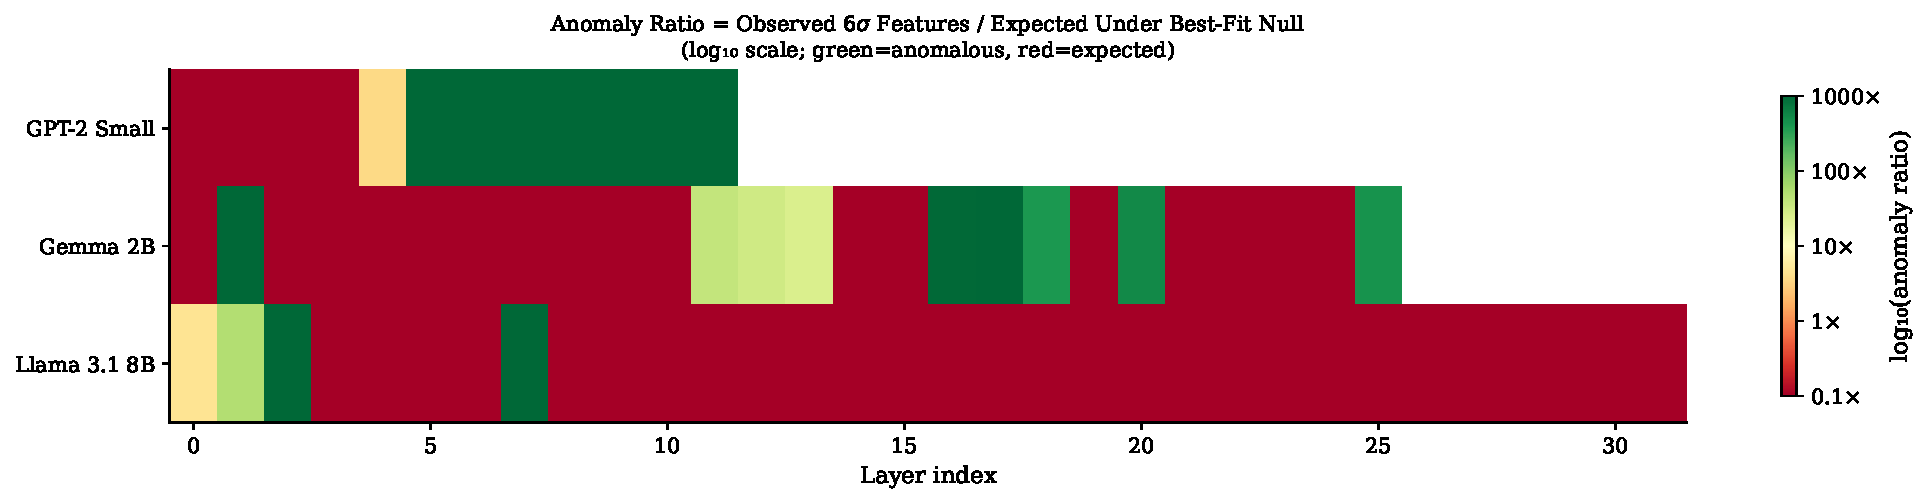
\includegraphics[width=0.95\textwidth]{../figures/phase1/anomaly_ratio_heatmap.pdf}
\caption{Log$_{10}$(anomaly ratio) = $\log_{10}(\text{observed}/\text{expected under winner model})$ per layer per model. Green = anomalous ($>10\times$), yellow = marginal ($2$--$10\times$), red = explained ($\sim 1\times$). Nearly all cells with$\geq 6\sigma$ features are strongly green. Llama L0 is the only marginal (yellow) case.}
\label{fig:heatmap}
\end{figure}

\begin{figure}[H]
\centering
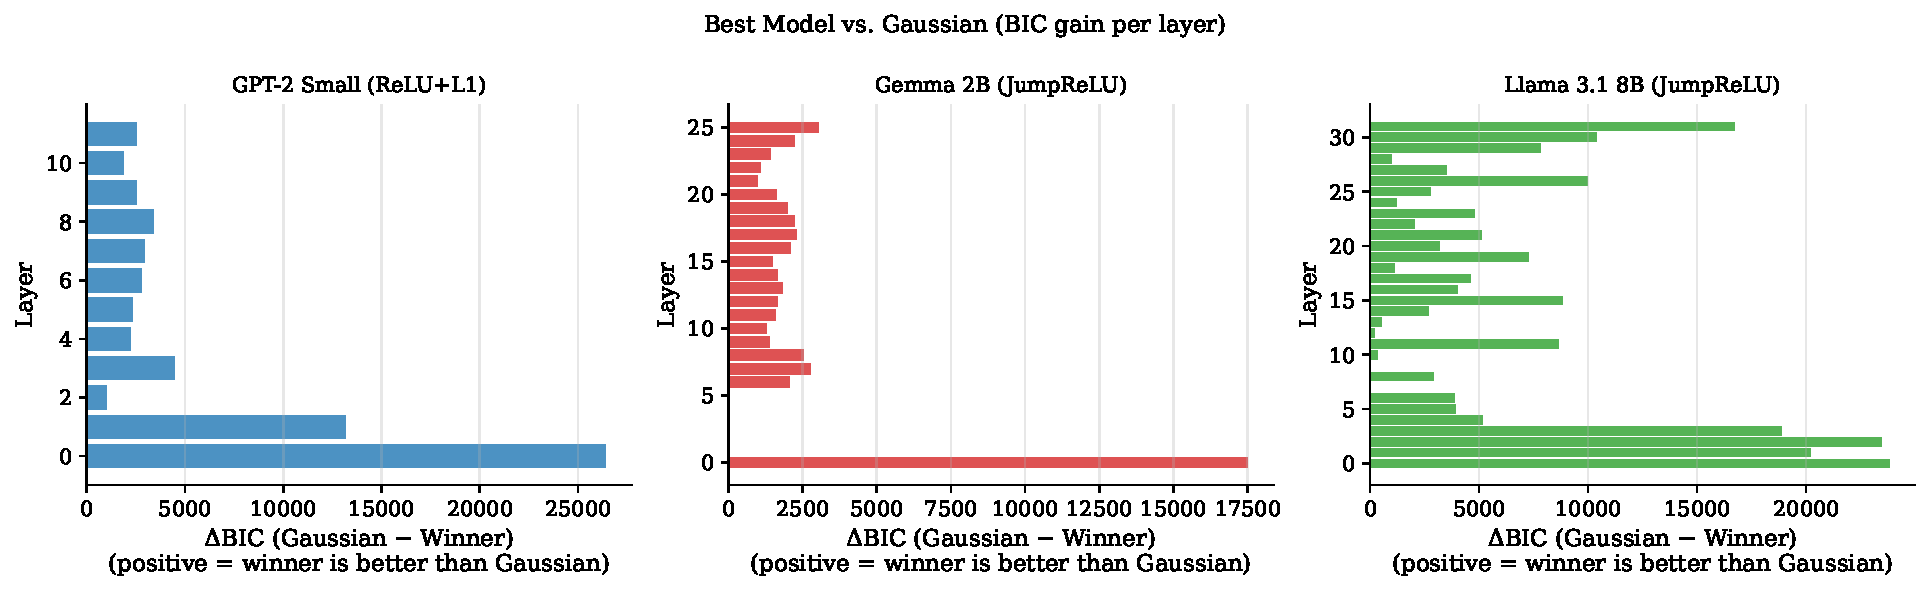
\includegraphics[width=0.90\textwidth]{../figures/phase1/bic_improvement_vs_gaussian.pdf}
\caption{BIC improvement over Gaussian for the winning model, per layer per model. Positive $\DBIC$ means the winner is better than Gaussian. Gaussian Mixture dominates, with especially large improvements in Llama early layers (L0: $\DBIC = 23{,}806$) and GPT-2 mid-late layers.}
\label{fig:bic}
\end{figure}

\begin{figure}[H]
\centering
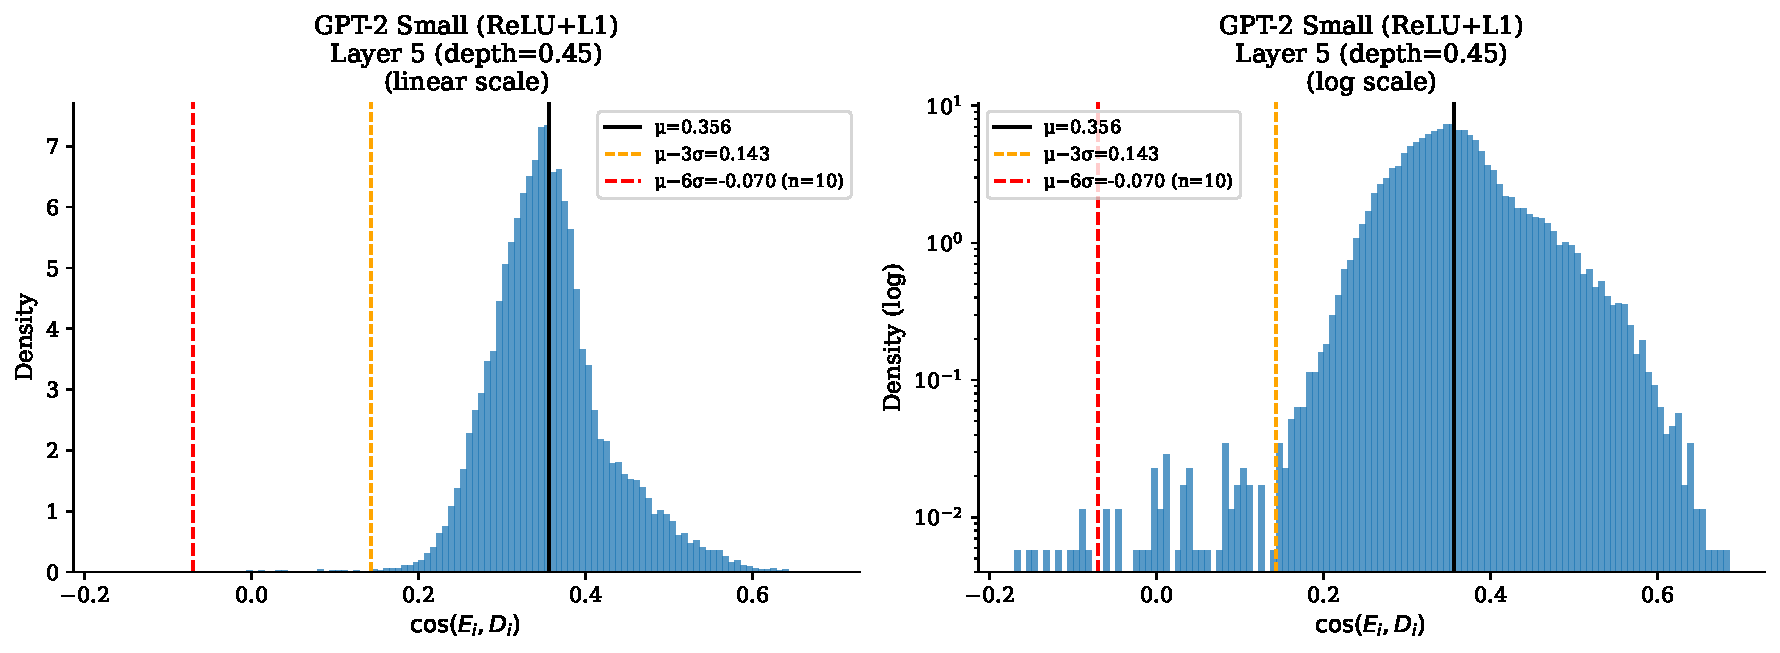
\includegraphics[width=0.95\textwidth]{../figures/phase1/hist_gpt2_L5.pdf}
\caption{GPT-2 Layer~5 (the layer with the most 6$\sigma$ features: 10). Log-scale histogram (right panel) makes the bimodal structure visible: a main peak near $\cosED \approx 0.36$ and a sparse tail extending to $-0.17$. Red dashed line marks the $\mu - 6\sigma$ threshold; 10 features lie below it. Under the Gaussian Mixture null, 0.005 are expected---a ratio of 1,944.}
\label{fig:gpt2_l5}
\end{figure}

\begin{figure}[H]
\centering
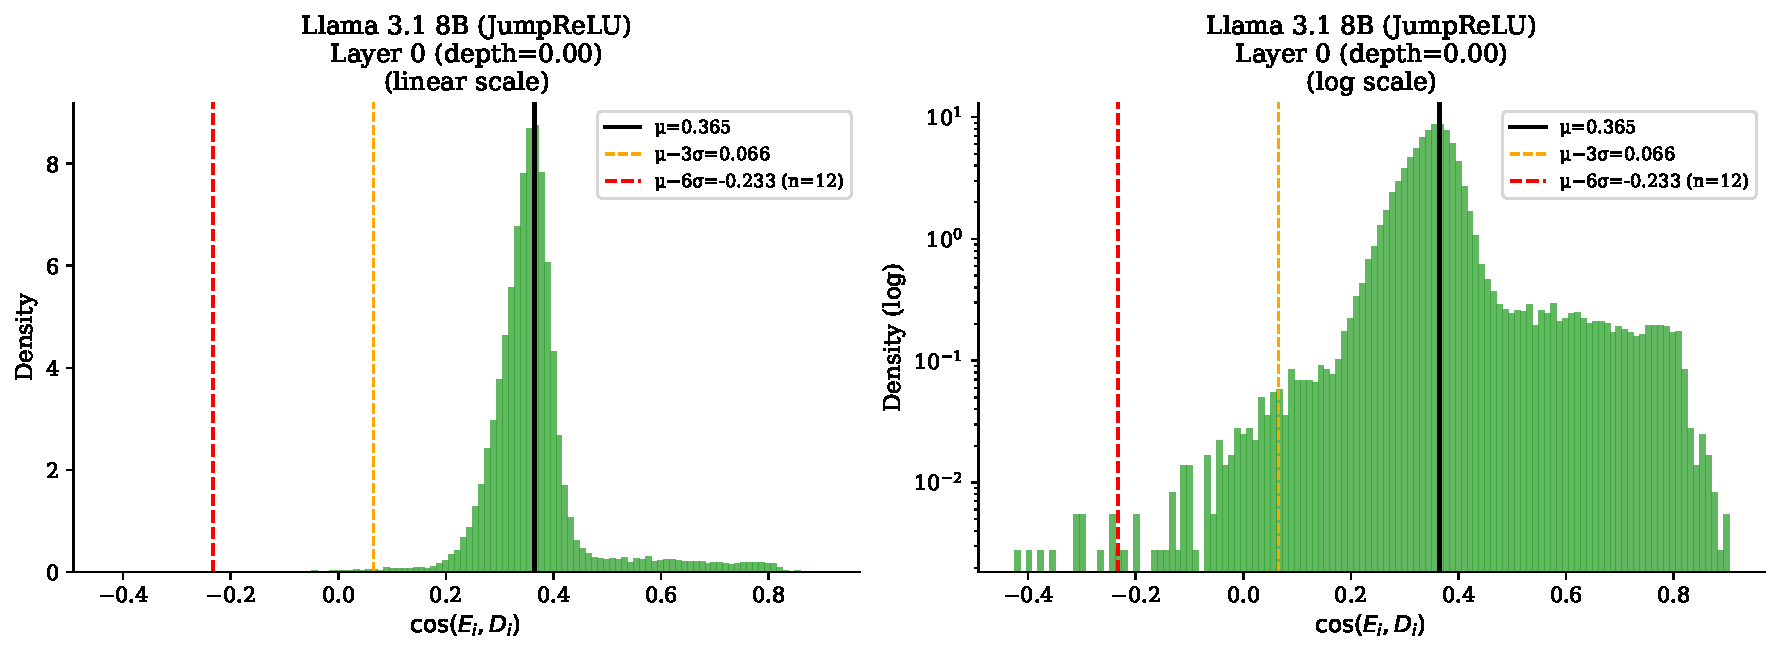
\includegraphics[width=0.95\textwidth]{../figures/phase1/hist_llama_L0.pdf}
\caption{Llama Layer~0. The log-scale histogram reveals a complex multi-modal structure: a bulk near $\cosED \approx 0.37$, a wide spread, and 12 features at $\leq -0.24$ (red dashed line, $\mu - 6\sigma$). Under Gaussian Mixture, 2.63 expected (ratio~$=$~4.6), placing this at G1-MARGINAL. The mixture captures the bimodal shape but not the full tail depth.}
\label{fig:llama_l0}
\end{figure}

\begin{figure}[H]
\centering
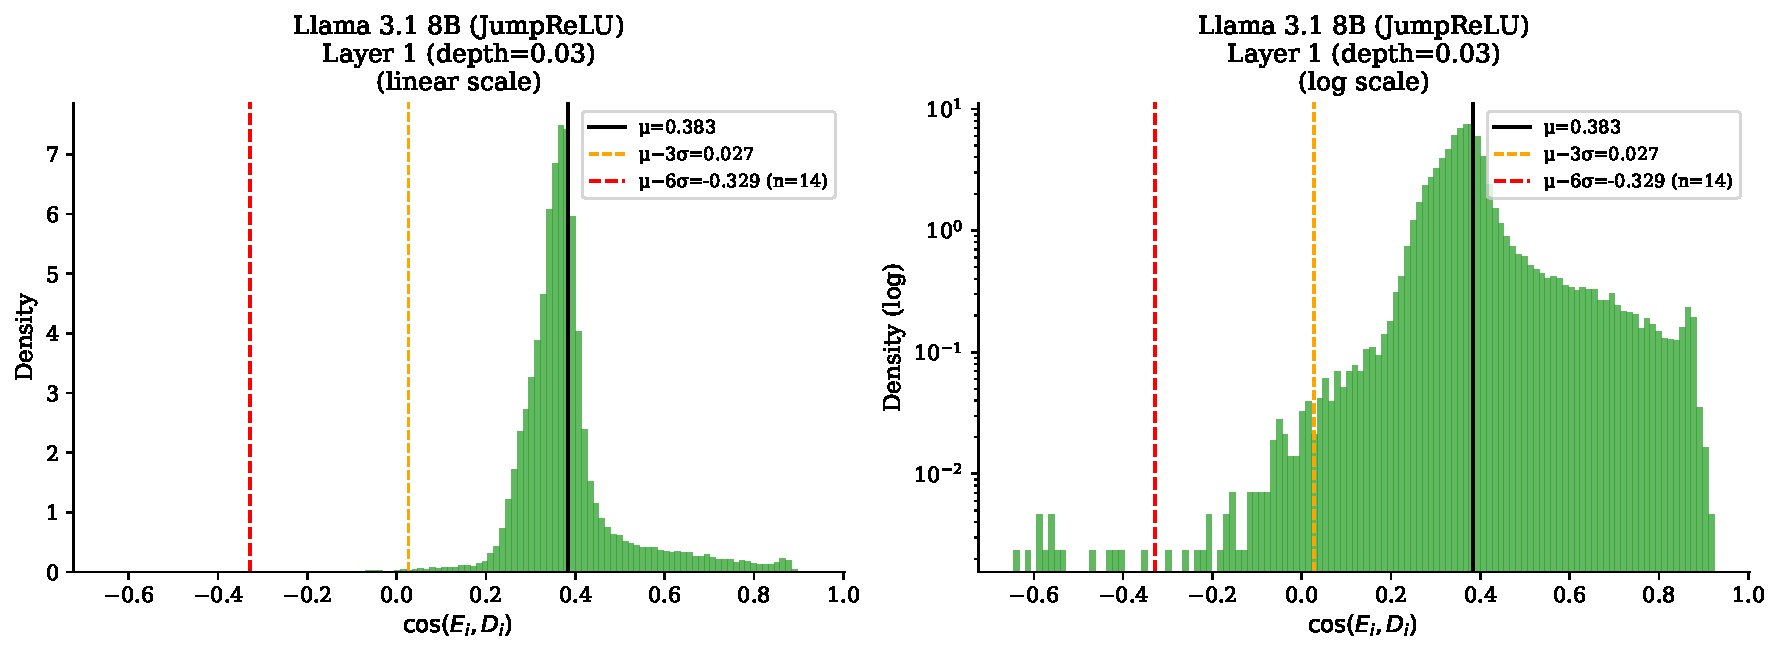
\includegraphics[width=0.95\textwidth]{../figures/phase1/hist_llama_L1.pdf}
\caption{Llama Layer~1. More clearly bimodal than L0. Under Gaussian Mixture, 0.29 features expected at the $6\sigma$ threshold; 14 observed (ratio~$=$~48.8). G1-YES. This confirms that Llama L1 anti-aligned features are genuinely anomalous beyond the bimodal structure.}
\label{fig:llama_l1}
\end{figure}

% ============================================================
\section{Gate G1 Decision}
\label{sec:gate}

\begin{gatedecision}{G1-YES --- GPT-2 Small (ReLU$+L_1$)}
\textbf{7 layers with $\geq 6\sigma$ features; all G1-YES.} \\
Maximum anomaly ratio: $10^{10}$ (Layer~9). Minimum: $3.6$ (Layer~4, G1-MARGINAL).\\
Winner model: Gaussian Mixture in 11/12 layers.\\
The anti-aligned features form a structurally distinct subpopulation, not a heavy-tailed extension of the bulk. Mechanistic investigation (Phases~2--4) is fully warranted.
\end{gatedecision}

\begin{gatedecision}{G1-YES --- Gemma 2B (JumpReLU)}
\textbf{9 layers with $\geq 6\sigma$ features; all G1-YES.}\\
Maximum anomaly ratio: $61{,}865$ (Layer~1). \\
\textit{Important caveat:} Gemma's anomalous features have $\cosED > 0$ (positive cosine). They are ``relatively anti-aligned'' (low vs.\ Gemma's high-alignment baseline) not ``absolutely anti-aligned.'' The claim from the original hypothesis---that anti-aligned features are mechanistically paradoxical ($\cosED < 0$)---applies only to GPT-2 and Llama, not Gemma.\\
Implication for Phase~4: co-activation analysis should focus on GPT-2 (and Llama), not Gemma.
\end{gatedecision}

\begin{gatedecision}{G1-YES --- Llama 3.1 8B (JumpReLU)}
\textbf{4 layers with $\geq 6\sigma$ features; 3 G1-YES, 1 G1-MARGINAL (L0).}\\
Maximum anomaly ratio: $336{,}065$ (Layer~2). Layer~1 ratio: $48.8$.\\
Layer~0 (G1-MARGINAL, ratio~$=$~4.6): the Gaussian Mixture partially explains the distribution's heavy tail, but 12 features remain in excess. The bimodal structure at L0 has a second component near the tail but not all the way to $-6\sigma$.\\
Mechanistic investigation of Llama L1 is warranted. L0 results should be interpreted cautiously.
\end{gatedecision}

\subsection{Effect on Subsequent Phases}

\paragraph{Phase~2 (Toy Model).} G1-YES for both GPT-2 and Llama confirms that anti-aligned features are genuine bimodal subpopulations (not noise) in both architectures. The toy model must address both mechanisms: L1-driven (GPT-2 late layers) and non-L1-driven (Llama early layers).

\paragraph{Phase~3 (Seed Stability).} The bimodal structure suggests the second Gaussian component is a real sub-population, not sampling noise. If the second component is stable across seeds, it strongly supports H1 or H3 depending on the component's location relative to the bulk.

\paragraph{Phase~4 (Co-activation Analysis).} Focus on:
\begin{itemize}[nosep]
  \item GPT-2 L5--L11: the primary G1-YES layers (14 features at $\leq\mu{-}6\sigma$ in L5, known absolutely negative cosine).
  \item Llama L1 (14 features, ratio=48.8): what activates these? Co-activation structure?
  \item Do NOT prioritize Gemma (positive-cosine anomalies are of a different nature).
\end{itemize}

\paragraph{Phase~5 (Architectural Comparison) -- Major revision.} The threshold architecture finding radically reorganizes Phase~5. The primary question is:
\begin{quote}
\emph{Does Gemma's per-feature threshold prevent the development of a structurally separated anti-aligned subpopulation?}
\end{quote}
Test: Gemma~9B (d\_model=$3{,584}$, 42 layers) should have per-feature thresholds (same architecture as Gemma~2B). If Gemma~9B also lacks absolute anti-alignment, size is not the explanation---architecture is. If Gemma~9B develops early-layer anti-alignment, the H6 size hypothesis (Phase~0) is supported.

% ============================================================
\section{Limitations}
\label{sec:limitations}

\paragraph{Gaussian Mixture initialization.} Mixture fitting used Nelder-Mead with 3 random initializations and 500 iterations. Local minima are possible; the reported winners may not be globally optimal mixtures. Future work should use EM with more initializations.

\paragraph{Gemma positive-cosine tail interpretation.} Classifying Gemma's $6\sigma$ features as ``anomalous'' uses a relative metric (sigma-distance from the mean). These features are not mechanistically paradoxical in the same sense as GPT-2/Llama's absolutely negative-cosine features. The statistical significance (G1-YES) reflects distributional anomaly, not necessarily mechanistic interest.

\paragraph{Llama architecture uncertainty.} The SAELens Llama release uses JumpReLU with scalar threshold, but the original Llama Scope paper describes TopK. The scalar threshold finding is robust (confirmed from weight files), but the comparison with Gemma requires caution about what ``JumpReLU with scalar threshold'' means functionally vs TopK.

\paragraph{Threshold measurement.} Thresholds were extracted from the SAE weight files as stored by SAELens. The raw Gemma~2B \texttt{params.npz} stores \texttt{log\_threshold}; we exponentiate to get $\theta_i = \exp(\log\theta_i)$. Our reported standard deviation ($\sigma_\theta \approx 0.37$) is in $\theta$ space, not log-space.

% ============================================================
\section{Conclusion}
\label{sec:conclusion}

Phase~1 delivers three major findings:

\begin{enumerate}
  \item \textbf{G1-YES for all three model families.} Anti-aligned features are genuinely anomalous under the best-fitting distributional null (typically Gaussian Mixture): ratios of $10^3$--$10^{10}$ for GPT-2, $38$--$61{,}865$ for Gemma~2B, and $4.6$--$336{,}065$ for Llama. The exception is Llama Layer~0 (G1-MARGINAL, ratio~$=$~4.6), which is partly explained by the bimodal structure but with some excess.

  \item \textbf{Bimodal structure, not heavy tails.} The Gaussian Mixture wins in 69\% of all layer-model pairs. The excess kurtosis observed in Phase~0 (up to 7.42 for Llama L0) is an artifact of bimodality, not a signature of a genuinely heavy-tailed unimodal process. This distinction matters: a bimodal interpretation implies a distinct mechanistic subpopulation, much stronger than a mere distributional artifact.

  \item \textbf{Threshold architecture asymmetry.} Gemma~2B's JumpReLU threshold is per-feature ($\sigma_\theta \approx 0.37$), while Llama's is effectively scalar ($\sigma_\theta \approx 10^{-7}$). This architectural difference is a primary candidate for explaining the Gemma--Llama alignment gap ($\mu \approx 0.75$ vs $0.48$) and should be the central investigation of Phase~5.
\end{enumerate}

The research program is confirmed to proceed. The mechanistic question---why do these structurally separated anti-aligned subpopulations exist, and what determines their depth-location?---remains fully open.

% ============================================================
\newpage
\appendix

\section{Complete Tail Anomaly Table}
\label{app:full_table}

\begin{longtable}{@{}lrrrrrrl@{}}
\caption{Full tail anomaly results. Only layers with $\text{observed} > 0$ shown.}\label{tab:full_tail}\\
\toprule
Model & L & $\mu$ & $\sigma$ & Winner & Obs & Exp & Ratio \\
\midrule
\endfirsthead
\toprule
Model & L & $\mu$ & $\sigma$ & Winner & Obs & Exp & Ratio \\
\midrule
\endhead
\bottomrule
\endfoot
% GPT-2
GPT-2 & L4  & 0.348 & 0.075 & Mixture & 2  & 0.550    & 3.6 \\
GPT-2 & L5  & 0.356 & 0.071 & Mixture & 10 & 0.005    & 1,944 \\
GPT-2 & L6  & 0.369 & 0.076 & Mixture & 6  & 0.0001   & 61,785 \\
GPT-2 & L7  & 0.379 & 0.078 & Mixture & 3  & 0.000012 & 254,370 \\
GPT-2 & L8  & 0.368 & 0.079 & Mixture & 4  & 0.0000086 & 464,698 \\
GPT-2 & L9  & 0.368 & 0.079 & Mixture & 1  & $<10^{-11}$ & $10^{10}$ \\
GPT-2 & L10 & 0.368 & 0.076 & Mixture & 3  & 0.000078 & 38,254 \\
GPT-2 & L11 & 0.349 & 0.074 & Mixture & 6  & 0.0018   & 3,316 \\
% Gemma
Gemma & L1  & 0.678 & 0.135 & Gaussian & 1 & 0.000016 & 61,865 \\
Gemma & L11 & 0.778 & 0.080 & Beta    & 3 & 0.079    & 38 \\
Gemma & L12 & 0.786 & 0.081 & Beta    & 3 & 0.101    & 30 \\
Gemma & L13 & 0.784 & 0.081 & Beta    & 2 & 0.084    & 24 \\
Gemma & L16 & 0.771 & 0.077 & Mixture & 1 & 0.0010   & 960 \\
Gemma & L17 & 0.765 & 0.080 & Mixture & 1 & 0.00022  & 4,609 \\
Gemma & L18 & 0.756 & 0.074 & Mixture & 1 & 0.0026   & 379 \\
Gemma & L20 & 0.765 & 0.073 & Mixture & 1 & 0.0020   & 512 \\
Gemma & L25 & 0.823 & 0.077 & Mixture & 4 & 0.0093   & 432 \\
% Llama
Llama & L0  & 0.365 & 0.100 & Mixture & 12 & 2.63 & 4.6 \\
Llama & L1  & 0.383 & 0.119 & Mixture & 14 & 0.29 & 48.8 \\
Llama & L2  & 0.414 & 0.134 & Mixture & 2  & $5.9\times10^{-6}$ & 336,065 \\
Llama & L7  & 0.490 & 0.161 & Gaussian & 1 & $3.2\times10^{-5}$ & 30,932 \\
\end{longtable}

\section{Reproducibility}
\label{app:repro}

\begin{verbatim}
# Execute Phase 1 analysis:
# from the repository root
python scripts/phase1_main.py

# Outputs:
#   results/phase1/cos_sim_*.npy          (raw arrays)
#   results/phase1/distributional_fits.csv (BIC/AIC per model per layer)
#   results/phase1/tail_pvalues.csv        (anomaly ratios)
#   results/phase1/threshold_stats.csv     (JumpReLU threshold statistics)
#   figures/phase1/*.{png,pdf}

# Software:
#   sae-lens==6.37.6, scipy, numpy, pandas, matplotlib
\end{verbatim}

% ============================================================
\newpage
\bibliographystyle{plainnat}
\begin{thebibliography}{6}

\bibitem[Bloom(2024)]{bloom2024}
Bloom, J. (2024). GPT2-Small-SAEs. HuggingFace: \texttt{jbloom/GPT2-Small-SAEs}.

\bibitem[He et~al.(2024)]{he2024}
He, Z., et~al. (2024). Llama Scope. \emph{arXiv:2410.20526}.

\bibitem[Leask et~al.(2025)]{leask2025}
Leask, P., et~al. (2025). Sparse Autoencoders Do Not Find Canonical Units. \emph{arXiv:2502.04878}.

\bibitem[Lieberum et~al.(2024)]{lieberum2024}
Lieberum, T., et~al. (2024). Gemma Scope. \emph{arXiv:2408.05147}.

\bibitem[Rajamanoharan et~al.(2024)]{rajamanoharan2024}
Rajamanoharan, S., et~al. (2024). JumpReLU SAEs. \emph{arXiv:2407.14435}.

\bibitem[Schwarz(1978)]{schwarz1978}
Schwarz, G. (1978). Estimating the Dimension of a Model. \emph{Ann.\ Statist.}\ 6(2), 461--464.

\end{thebibliography}

\end{document}
